\section{Problemstellungen und Lösungsansätze}

\subsection{REST}
\textit{Representational State Transfer (abgekürzt REST, seltener auch ReST) bezeichnet ein Programmierparadigma für verteilte Systeme, insbesondere für Webservices.}\vspace{5mm}\footnote{\url{https://de.wikipedia.org/wiki/Representational_State_Transfer (10.6.16)}}

REST verweist auf einige Prinzipien, die vorausgesetzt werden, damit der implementierte Service als RESTful bezeichnet werden kann. Bei den Prinzipien handelt es sich um: Client-Server, Zustandslosigkeit, Caching, eine Einheitliche Schnittstelle, Mehrschichtige Systeme und Code on Demand (optional). Im Zuge des Projekts wurde Wert darauf gelegt, dass das System diese Eigenschaften erfüllt.

\subsection{Überblick}

\begin{figure}[h]
	\centering
	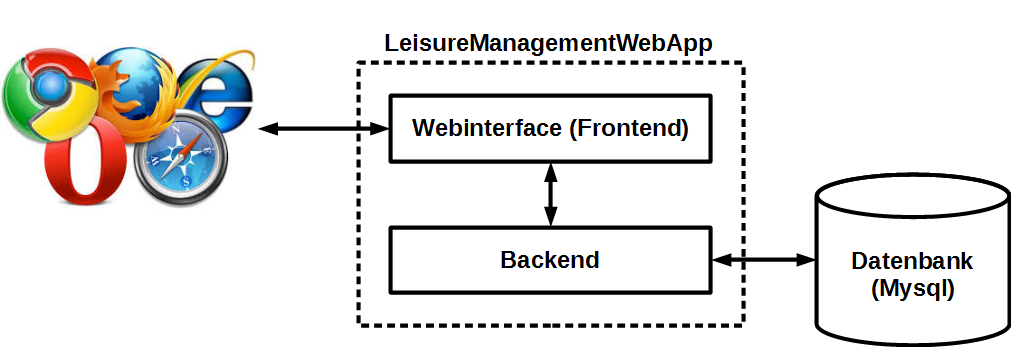
\includegraphics[width=0.7\linewidth]{2_solutions/pics/overview}
	\caption{Grober Design Überblick}
	\label{fig:overview}
\end{figure}

Wie die meisten Web-Applikationen besteht das Projekt aus einem Front- und einem Backend. Das Frontend (Client-Side) besteht aus einer Homepage, die von einem Browser aus aufgerufen wird. Es stellt eine Oberfläche zur Verfügung, mit deren Hilfe der Benutzer auf die Funktionalitäten der Applikation zugreifen kann. Das Frontend enthält jedoch nur Anzeige- und Transaktionslogik. Das bedeutet, dass es zwar Zugriff auf Funktionalitäten verschafft, und die Anzeigeelemente entsprechend der Benutzerinteraktion verändert, dann aber nur mittels eines http-Requests die entsprechenden Daten vom Backend anfordert und den zugehörigen Anzeigeelementen zuordnet. Die eigentliche Logik liegt im Backend (Server-Side). Es empfängt die Requests des Frontends, und sendet Daten als Antwort auf die Requests. So gut wie alle für die Organisation der Freizeit notwendigen Daten werden in einer Datenbank abgelegt. Das Backend fungiert auch als Schnittstelle zur Datenbank.   

\subsection{Backend: Spring MVC}
Das Backend wurde in Java implementiert. Hier wurde Spring MVC als unterstützendes Framework gewählt, da es einen sehr großen Funktionsumfang hat. Die beiden für dieses Projekt wichtigsten Features werden im Folgenden kurz beschrieben.

\subsubsection{Datenbank Anbindung}
Spring stellt mittels Spring-Data einige sehr praktische Werkzeuge zur Verfügung mit denen auf relationale Datenbanken zugegriffen werden kann. Es werden JPA-Schnittstellen zur Verfügung gestellt, die die Zuordnung und Übertragung von Objekten zu Datenbankeinträgen sehr stark vereinfachen.

\subsubsection{Datenübertragung}
Spring unterstützt außerdem einfache Wege, mittels denen URL's einfach auf Methoden gemappt werden können. Die empfangenen http-Requests können durch Lesen der URL- Parameter oder der Daten im http-Body in nutzbare Daten umgewandelt werden.

\subsection{Frontend: AngularJS/Javascript}
Zur Erstellung des Frontends wurde das JavaScript Framework AngularJS verwendet. AngularJS erweitert HTML um Attribute. Diese Attribute schaffen erstens eine sehr gute Schnittstelle zwischen den HTML-Elementen und der dahinter liegenden JavaScript Logik und zweitens ermöglichen sie eine dynamische Anpassung der HTML-Struktur des Basisdokuments.
